\documentclass{article}
\usepackage{tikz}
\usetikzlibrary{positioning, shapes.geometric, arrows.meta}
\usepackage[margin=1in]{geometry}

\title{Proposed Cloud-Based Data Flow for HE\textsuperscript{2}AT Center Post-Funding Restructure}
\author{}
\date{}

\begin{document}

\maketitle

\section*{Context and Purpose}
Due to NIH's withdrawal of funding for South African partners, the HE\textsuperscript{2}AT Center's data infrastructure must transition to a cloud-based solution (e.g., Azure). This document outlines a proposed data flow diagram indicating:
\begin{itemize}
    \item Levels of access for different HE\textsuperscript{2}AT partners
    \item Data ownership and control boundaries
    \item Data storage policies compliant with POPIA and GDPR
    \item Role of CeSHHAR and data access restrictions (e.g., date of birth)
    \item Long-term archival and use of de-identified data for future research
    \item Data security through geographic masking techniques
\end{itemize}

\section*{Data Access Roles and Responsibilities}
\begin{itemize}
    \item \textbf{Data Providers}: Retain ownership of Original Study Data. Data is stored in-region via secure transfer protocols and only accessed by the Core Data Team.
    \item \textbf{Core Data Team (UCT)}: Handles pre-processing, harmonisation, validation, and de-identification. Maintains audit logs, transformation records, and ensures metadata fidelity. Applies jittering and geographic aggregation methods.
    \item \textbf{Azure Cloud Platform}: Secure, compliant repository hosting geographically partitioned storage accounts with scalable role-based access control (RBAC).
    \item \textbf{HE\textsuperscript{2}AT Consortium (CeSHHAR, IBM, WHC, UPGC)}: Access to Consortium Shared Data, controlled via RBAC. No direct access to identifiable information.
    \item \textbf{External Researchers}: Access only fully de-identified datasets following DAC review, DTA signing, and full compliance audits.
\end{itemize}

\section*{Azure Cloud Technical Architecture}
\begin{itemize}
    \item \textbf{Geographically Scoped Storage}: Azure Storage Accounts are region-specific (e.g., South Africa North, West Europe) to comply with POPIA and GDPR.
    \item \textbf{Data Containers}: Containers are separated for raw, harmonised, and de-identified data by project, access level, and jurisdiction.
    \item \textbf{Access Levels}:
    \begin{itemize}
        \item Level 0: Original Study Data (Core Data Team only)
        \item Level 1: Consortium Shared Data (HE\textsuperscript{2}AT Consortium via RBAC)
        \item Level 2: RP1/RP2 De-identified Data (DAC-approved)
        \item Level 3: Inferential Data (open, non-identifiable aggregates)
    \end{itemize}
    \item \textbf{Access Management}: Azure Active Directory manages RBAC tiers. Conditional access restricts login by IP, geolocation, and 2FA.
    \item \textbf{Encryption and Compliance}: AES-256 encryption, TLS in transit. Azure Key Vault secures key lifecycle. Meets NIST and ISO standards.
    \item \textbf{Monitoring and Auditing}: Continuous tracking via Azure Monitor, Log Analytics, and Sentinel with incident alerts.
\end{itemize}

\section*{Data Security and Jittering Techniques}
\begin{itemize}
    \item \textbf{Geographic Aggregation}: Data aggregated to census small areas or wards to reduce re-identification risk.
    \item \textbf{Location Jittering}: Gaussian displacement used to obfuscate coordinates, respecting local population density and spatial k-anonymity.
    \item \textbf{Expert Review}: Geo-masking approaches reviewed by a technical committee from UCT, IBM, and NIH.
\end{itemize}

\section*{Data Use and DTA Structure}
\begin{itemize}
    \item \textbf{Data Use}: De-identified datasets may be reused for future research projects under ethical clearance and DAC oversight.
    \item \textbf{DTA Framework}: All DTAs will specify:
    \begin{itemize}
        \item Dataset scope and project affiliation
        \item Region of storage and compliance standards
        \item Permitted duration and modality of access
        \item Non-transfer clauses and audit rights
    \end{itemize}
\end{itemize}

\section*{Data Flow Diagram Overview}
\textit{The diagram below will be further translated into XML/Draw.IO for presentation.}

\begin{center}
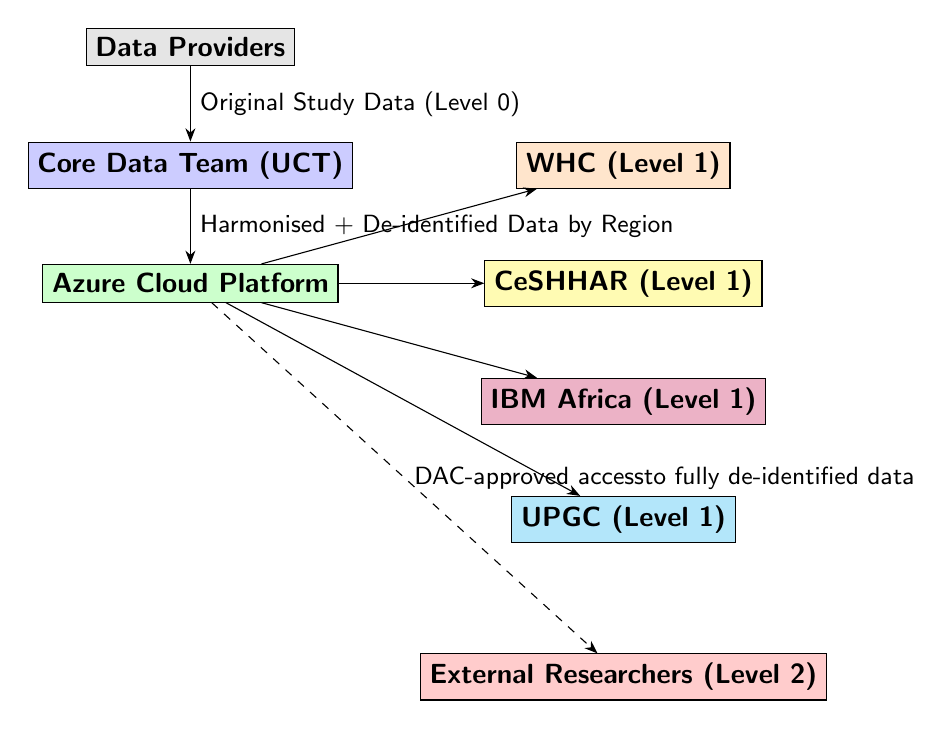
\begin{tikzpicture}[node distance=1.5cm and 2.5cm, on grid, every node/.style={font=\sffamily}, >=Stealth]
  \node[draw, rectangle, fill=gray!20] (provider) {\textbf{Data Providers}};
  \node[draw, rectangle, fill=blue!20, below=of provider] (core) {\textbf{Core Data Team (UCT)}};
  \node[draw, rectangle, fill=green!20, below=of core] (cloud) {\textbf{Azure Cloud Platform}};

  \node[draw, rectangle, fill=yellow!30, right=of cloud, xshift=3cm] (cesshar) {\textbf{CeSHHAR (Level 1)}};
  \node[draw, rectangle, fill=orange!20, above=of cesshar] (whc) {\textbf{WHC (Level 1)}};
  \node[draw, rectangle, fill=purple!30, below=of cesshar] (ibm) {\textbf{IBM Africa (Level 1)}};
  \node[draw, rectangle, fill=cyan!30, below=of ibm] (upgc) {\textbf{UPGC (Level 1)}};
  \node[draw, rectangle, fill=red!20, below=of upgc, yshift=-0.5cm] (external) {\textbf{External Researchers (Level 2)}};

  \draw[->] (provider) -- node[right] {\small Original Study Data (Level 0)} (core);
  \draw[->] (core) -- node[right] {\small Harmonised + De-identified Data by Region} (cloud);
  \draw[->] (cloud) -- (whc);
  \draw[->] (cloud) -- (cesshar);
  \draw[->] (cloud) -- (ibm);
  \draw[->] (cloud) -- (upgc);
  \draw[->, dashed] (cloud) -- node[right, align=left] {\small DAC-approved access \newline to fully de-identified data} (external);
\end{tikzpicture}
\end{center}

\section*{Key Notes for Data Providers}
\begin{itemize}
    \item Data ownership remains with the original provider.
    \item DTAs ensure transparent roles, rights, and revocability.
    \item Regional isolation prevents unlawful cross-border data transfer.
    \item Data is stored, accessed, and used under secure, compliant, and ethically reviewed protocols.
    \item Extended future use of de-identified datasets is possible, always under DAC oversight and updated ethical approval.
\end{itemize}

\end{document} 